
Ce chapitre a pour objectif d'interpréter les résultats présentés lors de la validation expérimentale. Les différents essais permettent de comparer le comportement réel de la maquette avec celui prédit par le modèle physique et les simulations. Les écarts observés sont analysés afin d'identifier leurs origines et d'évaluer les limites de la modélisation.
\section{Analyse des résultats}
\subsection{Mesures modèle physique}

\subsubsection{Chute libre}

Les essais de chute libre montrent une bonne concordance entre les résultats expérimentaux et les simulations. Pour les deux conditions initiales étudiées, les courbes d'évolution de l'angle présentent une dynamique similaire, ce qui valide le modèle mécanique développé.

On observe toutefois que l'évolution de l'angle mesuré est légèrement plus lente que celle prédite par la simulation. Cet écart peut s'expliquer par des phénomènes qui n'ont pas été entièrement pris en compte dans le modèle, notamment les frottements de roulement entre les roues et le sol ainsi que le couple résistant généré par les moteurs pas à pas lorsqu'ils sont entraînés mécaniquement. En effet, même lorsque les moteurs ne sont pas commandés, leur réluctance magnétique produit un couple de retenue qui s'oppose au mouvement et ralentit la chute du système.

Malgré ces écarts, la bonne superposition des courbes montre que le modèle physique reproduit correctement le comportement global de la maquette et constitue une représentation suffisamment fidèle pour la conception et le réglage de la commande.
\subsubsection{Vitesse maximale}

La vitesse maximale mesurée est de

\[
v_{max}=0.864~\si{\meter\per\second}.
\]

Avec un rayon de roue de

\[
r=0.055~\si{\meter},
\]

la vitesse angulaire correspondante vaut

\[
\omega=\frac{v}{r}
=\frac{0.864}{0.055}
\simeq15.7~\si{\radian\per\second}
\approx5\pi~\si{\radian\per\second}.
\]

Cette valeur correspond à la limitation logicielle implémentée dans le contrôleur.

La concordance entre la valeur théorique et la mesure expérimentale confirme que cette limitation est correctement appliquée.

\subsubsection{Angle maximal}

Les essais montrent que les moteurs sont désactivés dès que l'inclinaison atteint la valeur limite de $30^\circ$. Cette désactivation provoque une chute immédiate de la vitesse à une valeur nulle.

Ce comportement confirme le bon fonctionnement de la protection logicielle. 

\subsubsection{Régulation de maintien}

Les essais de maintien mettent en évidence le bon fonctionnement de la boucle de régulation.

Lorsqu'une perturbation est appliquée manuellement au robot, celui-ci génère immédiatement une correction destinée à ramener son centre de gravité au-dessus du point de contact avec le sol.

Le comportement observé traduit un compromis satisfaisant entre rapidité de correction et stabilité. Les gains du correcteur permettent de limiter les dépassements tout en assurant un temps de réponse relativement court (< 1s).

Les réponses obtenues pour les perturbations positives et négatives présentent des caractéristiques similaires, ce qui confirme la symétrie du comportement du système.

\subsubsection{Déplacement trapézoïdal}

Les essais de déplacement montrent que le profil de vitesse généré par le contrôleur est correctement suivi durant la phase d'accélération. La vitesse augmente de manière linéaire jusqu'à atteindre la valeur de consigne avant de rester pratiquement constante pendant la phase de déplacement uniforme.

Une différence apparaît toutefois durant la phase de décélération. La vitesse mesurée décroît plus rapidement la vitesse simulée, ce qui indique que le système freine davantage que prévu par le modèle.

Cette différence se répercute sur la position finale. La simulation prévoit un déplacement de $2.985~\si{\meter}$ tandis que la mesure expérimentale atteint $2.854~\si{\meter}$, soit une erreur relative d'environ $4.4\,\%$.

Cet écart reste modéré et s'explique principalement par les simplifications du modèle, les frottements mécaniques qui ne sont pas représentés dans la simulation, ainsi que les variations du contact entre les roues et le sol.

La comparaison entre les roues en aluminium et les roues en PLA met également en évidence l'influence du matériau sur le comportement dynamique du système. La simulation montre une avance de la réponse en vitesse pour les roues en PLA, tendance qui est également observée expérimentalement. Les roues en aluminium présentent toutefois un comportement plus stable, avec un signal de vitesse moins bruité. Cette meilleure régularité s'explique par la rigidité supérieure du matériau, limitant les déformations de la roue lors du déplacement.

Cependant, les roues en PLA présentent un meilleur suivi moyen de la consigne de vitesse. Malgré un niveau d'oscillation plus important sur la mesure instantanée, elles présentent un retard plus faible lors des phases transitoires, notamment pendant l'accélération. Ce comportement peut notamment s'expliquer par une inertie plus faible des roues en PLA, permettant au système d'atteindre plus rapidement la vitesse demandée.

Ainsi, le choix du matériau représente un compromis entre stabilité de la réponse et précision du suivi dynamique. Les roues en aluminium permettent d'obtenir une réponse plus régulière et moins sensible au bruit, tandis que les roues en PLA offrent un comportement moyen plus proche de la consigne imposée. Dans le cadre de cet essai, les différences observées restent toutefois limitées, les deux configurations permettant de réaliser correctement le déplacement demandé.
\subsubsection{Influence de l'IMU}

Les essais mettent en évidence deux phénomènes liés aux mesures de l'IMU.

Le premier concerne le positionnement du capteur dans la structure. Les mesures montrent que la position de l'IMU influence directement l'évolution de l'angle estimé. Plus le capteur est éloigné du centre de rotation, plus les accélérations linéaires mesurées sont importantes, ce qui modifie l'estimation de l'inclinaison.

Le second phénomène apparaît lors des accélérations brusques. Lorsqu'une impulsion est appliquée au système, l'angle estimé évolue tout d'abord dans une direction opposée au sens de la poussée avant de revenir progressivement vers sa valeur d'équilibre. Ce comportement s'explique par le principe même de fonctionnement de l'accéléromètre, qui mesure simultanément l'accélération gravitationnelle et les accélérations dues au mouvement.

Pendant la phase d'accélération, ces deux contributions ne peuvent plus être distinguées, ce qui perturbe temporairement l'estimation de l'angle. Une fois l'accélération terminée, le filtre de fusion retrouve progressivement une estimation cohérente et l'angle revient vers sa valeur réelle.

Dans l'ensemble, ces essais montrent que les perturbations observées ne proviennent pas d'une erreur de la régulation mais des limites physiques de la mesure inertielle.

\subsection{Utilisabilité}

Le système présente une bonne utilisabilité. La charge du robot est facilitée par sa conception, permettant une manipulation aisée lors des phases de désassemblage et d'assemblage. L'interface utilisateur développée sous forme d'\acrshort{pwa} est intuitive et rapidement prise en main, permettant un contrôle efficace du système.

Les protections prévues pour amortir les chutes remplissent correctement leur fonction et limitent les risques d'endommagement du robot lors des pertes d'équilibre. De plus, les roues peuvent être retirées facilement, ce qui simplifie le transport du système et réduit son encombrement.
\subsection{Mesures électriques}

Les mesures réalisées mettent en évidence une bonne concordance entre les tensions théoriques et les tensions mesurées. Les alimentations de $5\,\si{\volt}$ et de $3.3\,\si{\volt}$ présentent des écarts inférieurs à quelques dizaines de millivolts, ce qui confirme le bon fonctionnement des convertisseurs et régulateurs présents sur la carte.

En revanche, les puissances mesurées sont systématiquement inférieures aux estimations théoriques établies lors du dimensionnement. Cette différence provient en premier lieu de l'hypothèse retenue pour la consommation de l'ESP32. Afin de garantir un dimensionnement conservatif de l'alimentation, le courant maximal indiqué dans la documentation technique, soit $400\,\si{\milli\ampere}$, a été utilisé. Cette hypothèse correspond au pire cas de fonctionnement (« \textit{worst-case scenario} ») et conduit à une puissance théorique d'environ $2\,\si{\watt}$. En pratique, la consommation du microcontrôleur est nettement plus faible, ce qui explique que la puissance totale mesurée du système soit inférieure à la valeur calculée lorsque les moteurs sont désactivés.

Une seconde différence importante concerne la consommation des moteurs pas à pas. Les calculs théoriques supposent que le courant nominal est appliqué en permanence dans les enroulements afin de fournir le couple maximal. Or, le pilote TMC2226 met en œuvre une régulation intelligente du courant et adapte en permanence celui-ci aux besoins réels du moteur. Lorsque le couple demandé est faible ou lorsque le moteur est maintenu à l'arrêt, le courant effectivement délivré est significativement réduit. Cette gestion dynamique permet de diminuer les pertes Joule dans les enroulements et explique que les puissances mesurées, aussi bien à vitesse nulle qu'à vitesse maximale, soient sensiblement inférieures aux valeurs théoriques.

De plus, les mesures expérimentales ont été réalisées avec les roues de la maquette hors contact avec le sol. Les moteurs n'avaient donc pas à fournir le couple nécessaire au déplacement de la structure ni à vaincre les efforts liés au frottement et à la charge mécanique. La charge appliquée aux moteurs étant ainsi fortement réduite, le courant réellement consommé par les pilotes est inférieur à celui attendu lors d'une utilisation en conditions réelles. Les puissances mesurées correspondent donc à un fonctionnement à vide des moteurs et constituent une estimation optimiste de la consommation en déplacement.

Les mesures expérimentales montrent ainsi que le dimensionnement électrique réalisé est volontairement conservatif. Les hypothèses retenues lors de la conception garantissent que l'alimentation reste correctement dimensionnée dans les conditions les plus défavorables, tandis que la consommation réelle de la maquette demeure inférieure grâce à la gestion efficace de l'énergie par les différents composants électroniques, en particulier le pilote TMC2226.
L'autonomie de la maquette est estimée à partir de l'énergie disponible dans la batterie et de la puissance consommée :

\begin{equation}
    t = \frac{E}{P}
\end{equation}

où \(E=\SI{19.24}{\watt\hour}\) est l'énergie stockée dans la batterie.

En utilisant les puissances mesurées :

\begin{itemize}
    \item À vitesse nulle (\(P_{tot}=\SI{2.66}{\watt}\)) :
    \begin{equation}
        t_{\text{repos}}=\frac{19.24}{2.66}=7.23\,\si{\hour}
    \end{equation}

    \item À vitesse maximale (\(P_{tot}=\SI{8.89}{\watt}\)) :
    \begin{equation}
        t_{\text{max}}=\frac{19.24}{8.89}=2.16\,\si{\hour}
    \end{equation}
\end{itemize}

L'autonomie de la maquette est donc comprise entre environ \SI{2.2}{\hour} dans les conditions les plus exigeantes et \SI{7.2}{\hour} lorsque les moteurs sont à l'arrêt. En pratique, lors d'une utilisation normale avec des vitesses variables, l'autonomie réelle se situera entre ces deux valeurs.

\section{Guide d'utilisation}
Afin de pouvoir contrôler la maquette, la procédure à suivre est la suivante:
\begin{enumerate}
    \item Mettre le système sous tension à l'aide de l'interrupteur \texttt{SW1}.
    \item Établir une connexion au réseau WiFi: \texttt{self-balancing-bot} en utilisant le mot de passe: \texttt{123456789}.
    \item Accéder à l'interface utilisateur via un navigateur web en se connectant à l'adresse \texttt{192.168.4.1}.
    \item Ajouter l'application à l'écran d'accueil du périphérique mobile à l'aide de la fonction de partage du navigateur.
    \item Lancer l'application depuis l'écran d'accueil afin d'accéder à l'interface de commande du module.
\end{enumerate}

Il est imporant de noter ici que pour la charge de la batterie, le système doit d'abord être mis hors tension avec l'interrupteur \texttt{SW1}, ensuite, la batterie est débranchée puis chargée.

Le courant de charge est généralement exprimé en fonction de la capacité nominale de la batterie, sous la forme d'un taux de charge en \emph{C}. Dans ce cas, un courant de $1\,\mathrm{A}$ correspond à un taux de charge de :
\[
\frac{1\,\mathrm{A}}{1.3\,\mathrm{Ah}} \approx 0.77\,C
\]
Ce taux reste inférieur à une charge à $1\,C$, soit environ $1.3\,\mathrm{A}$ pour cette batterie, et permet de limiter l'échauffement ainsi que la dégradation prématurée des cellules.

Une charge avec un courant supérieur à $1\,\mathrm{A}$ augmenterait les contraintes électrochimiques sur les cellules LiPo, pouvant entraîner une élévation excessive de la température, une diminution de la durée de vie de la batterie ou, dans des conditions défavorables, un risque de gonflement ou d'endommagement des cellules. La limitation à $1\,\mathrm{A}$ constitue donc un compromis entre le temps de charge et la préservation de la sécurité et de la durée de vie de la batterie.


\section{Améliorations possibles}

Plusieurs améliorations pourraient être envisagées afin de poursuivre le développement et d'améliorer les performances du système étudié.

Une première amélioration concernerait la modélisation du système. Le modèle de simulation pourrait être complété en intégrant davantage de phénomènes physiques comme les pertes du au contact entre les roues et le sol. Une modélisation plus précise permettrait de réduire l'écart observé entre les résultats simulés et expérimentaux.

Une autre amélioration possible serait l'implémentation d'un système de régulation de type \acrshort{lqr} (\textit{Linear Quadratic Regulator}). Contrairement à une approche classique basée sur plusieurs correcteurs \acrshort{pid} indépendants, le régulateur \acrshort{lqr} considère l'ensemble du système dynamique et calcule directement une commande optimale à partir de l'état complet du robot.

\section{Utilisation de l'IA}

Dans le cadre de ce rapport, l'IA a été utilisée uniquement comme une aide à la rédaction. Le modèle utilisé est ChatGPT basé sur GPT-4 . L'ensemble des concepts et des idées présentés dans ce rapport ont été développés \textbf{sans l'aide de l'IA}.

\section{Conclusion personnelle}
La réalisation de ce projet a été une expérience particulièrement enrichissante. Elle m'a permis de mettre en pratique les connaissances acquises durant ma formation, tout en découvrant les différentes étapes nécessaires au développement complet d'un système robotique, de sa conception jusqu'à sa validation expérimentale.

Ce travail m'a permis d'approfondir mes compétences dans de nombreux domaines techniques, notamment la modélisation et la conception 3D, la fabrication mécanique, la conception de cartes électroniques (\acrshort{pcb}), la programmation en C++, le développement d'un serveur Web ainsi que l'intégration de l'ensemble de ces éléments au sein d'un robot fonctionnel.

La réalisation de ce projet m'a également sensibilisé aux contraintes liées au développement d'un système réel. Contrairement à une approche uniquement théorique, la fabrication d'un robot nécessite de prendre en compte de nombreux paramètres tels que les limitations des composants et les écarts entre la simulation et la réalité expérimentale.

Les phases de tests et d'analyse des résultats m'ont permis de mieux comprendre l'importance d'une démarche expérimentale rigoureuse et de l'amélioration progressive d'un système. La comparaison des différentes solutions mécaniques, notamment l'étude de l'influence du matériau des roues, a également montré l'impact des choix de conception sur les performances finales du robot.
Je tiens à remercier le centre de formation de la base aérienne de Payerne pour son soutien dans la réalisation de ce projet, notamment pour l'usinage des jantes en aluminium. Je remercie également le Makelab pour la fabrication des deux pièces latérales découpées au laser ainsi que pour les moyens mis à disposition.

Je souhaite également remercier mon professeur accompagnant, M. Girardin Michel, pour son suivi, ses conseils et son accompagnement tout au long de la réalisation de ce projet.

Enfin, je remercie mon relecteur, Ding Lionel, pour le temps consacré à la relecture de ce travail ainsi que pour ses remarques constructives ayant permis d'améliorer la qualité de ce rapport.


\vspace{2cm}

\begin{flushright}
    Yverdon-les-bains, le \today
    
    \vspace{1cm}
    
    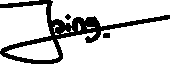
\includegraphics[width=4cm]{assets/figures/signature.pdf}\\
    \vspace{0.2cm}
    Ding Jérémy
\end{flushright}